La suite $\suiten$ est définie sur $\N$ par $u_0=1$ et pour tout entier naturel $n$, $$u_{n+1}=  \dfrac34 u_n+\dfrac14 n+1.$$

\begin{enumerate}
	\item Calculer, en détaillant les calculs, $u_1$ et $u_2$ sous forme de fraction irréductible.
\end{enumerate}

L’extrait, reproduit ci-dessous, d’une feuille de calcul réalisée avec un tableur présente les valeurs des premiers termes de la suite $\suiten$.

\begin{center}
	\begin{tikzpicture}
		\tableur[6]{A-B}
		\celtxt*[c]{A}{1}{$n$}
		\celtxt*[c]{B}{1}{$u_n$}
		\celtxt*[c]{A}{2}{$0$}
		\celtxt*[c]{A}{3}{$1$}
		\celtxt*[c]{A}{4}{$2$}
		\celtxt*[c]{A}{5}{$3$}
		\celtxt*[c]{A}{6}{$4$}
		\celtxt*[c]{B}{2}{$1$}
		\celtxt*[c]{B}{3}{$1,75$}
		\celtxt*[c]{B}{4}{$2,5625$}
		\celtxt*[c]{B}{5}{$3,421875$}
		\celtxt*[c]{B}{6}{$4,31640625$}
	\end{tikzpicture}
\end{center}

\begin{enumerate}[resume]
	\item 
	\begin{enumerate}
		\item Quelle formule, étirée ensuite vers le bas, peut-on écrire dans la cellule {\helvbx B3} de la feuille de calcul pour obtenir les termes successifs de $\suiten$ dans la colonne {\helvbx B} ?
		\item Conjecturer le sens de variation de la suite $\suiten$.
	\end{enumerate}
	\item 
	\begin{enumerate}
		\item  Démontrer par récurrence que, pour tout entier naturel $n$, on a : $n \leqslant u_n \leqslant n+1$.
		\item En déduire, en justifiant la réponse, le sens de variation et la limite de la suite $\suiten$.
		\item Démontrer que : \[\lim_{n \to +\infty} \dfrac{u_n}{n} = 1.\]
	\end{enumerate}
	\item On désigne par $\suiten[v]$ la suite définie sur $\N$ par $v_n= u_n-n$.
	\begin{enumerate}
		\item Démontrer que la suite $\suiten[v]$ est géométrique de raison $\dfrac34$.
		\item En déduire que, pour tout entier naturel $n$, on a : $u_n=\left(\dfrac34\right)^n+n$.
	\end{enumerate}
\end{enumerate}

